\paragraph*{稀疏波}

\PDEIndexMark{idx:system-rarefaction-introduction}现在构造一个连续波族, 推广单个守恒律的稀疏波. 与激波情形一样, 将证明从左状态 $\bm{u}^l$ 出发的 $n$ 条曲线的存在性, 它们给出可由单个稀疏波直接连接的所有可能的右状态 $\bm{u}^r$.

总体思想基于单个守恒律的构造. 假设对某个 $k=1,2,\ldots,n$ 有
\begin{equation}\label{eq:rarefaction-increasing-characteristic-speed}
\lambda_k(\bm{u}^l)<\lambda_k(\bm{u}^r).
\end{equation}
Lax 条件立即排除了用单个激波连接这两个状态的可能性. 现在仿照单个方程情形的过程, 画出从原点左侧与右侧出发的特征线 $x=\lambda(\bm{u}^l)t$ 和 $x=\lambda(\bm{u}^r)t$. (注意, 对方程组而言, 解不一定沿特征线为常数, 但在此情形下, 这样的"猜测"会导出一个解.) 这一特征线图与 Figure~\ref{fig:characteristic-gap} 非常相似: 在 $(x,t)$ 平面的上半部分有两个被特征线覆盖的区域, 中间留有一个楔形空白区域. 若顺势将解定义为在左侧阴影区域取常数 $\bm{u}^l$, 在右侧区域取 $\bm{u}^r$, 应如何填补空白区域? 答案是可使用以下类型的波.

\begin{Definition}
\label{def:system-simple-wave}
设 $\bm{u}$ 为区域 $D$ 内守恒律 \eqref{eq:conservation-law-system} 的一个 $C^1$ 解. 若所有 $k$-Riemann 不变量在 $D$ 内都为常数, 则称 $\bm{u}$ 为 \textbf{k-稀疏波} (或 \textbf{k-简单波}).
\end{Definition}

正如从单个守恒律的结果所能期待的, 若能找到填满空白楔形区域的稀疏波, 则对应于 $\lambda_k$ 的特征线形成一个"扇形".

\begin{Theorem}
\label{thm:system-rarefaction-straight-characteristics}
设 $\bm{u}$ 为区域 $D$ 内的 $k$-稀疏波. 那么特征曲线 $\hat x'(t)=\lambda_k(\bm{u}(\hat x(t),t))$ 是直线, 且 $\bm{u}$ 沿这些直线为常数.
\end{Theorem}

\begin{Proof}
需要证明
\begin{equation}\label{eq:rarefaction-constant-along-characteristics}
0=\dfrac{\mathrm{d}}{\mathrm{d}t}\bm{u}(\hat x(t),t)=\bm{u}_t+\lambda_k\bm{u}_x.
\end{equation}
Lemma~\ref{lem:riemann-invariants-existence} 断言存在 $n-1$ 个 $k$-Riemann 不变量 $w_i$, $i=1,2,\ldots,n-1$, 其梯度线性无关. 由于 $\bm{u}$ 为 $k$-稀疏波, $w_i(\bm{u}(x,t))$ 为常数, 因而
\begin{equation}\label{eq:rarefaction-invariant-directional-derivatives}
\dfrac{\mathrm{d}}{\mathrm{d}t}w_i(\bm{u}(\hat x(t),t))=\nabla w_i\cdot(\bm{u}_t+\lambda_k\bm{u}_x)=0,
\end{equation}
其中 $i=1,2,\ldots,n-1$. 利用 $\bm{u}$ 解方程 \eqref{eq:conservation-law-system} 这一事实及 $\bm{l}_k$ 的定义, 推出
\begin{equation}\label{eq:rarefaction-left-eigenvector-identity}
\bm{l}_k\cdot(\bm{u}_t+\lambda_k\bm{u}_x)=\bm{l}_k\cdot(\bm{u}_t+\nabla\bm{f}\bm{u}_x)=0.
\end{equation}
因此, $\bm{u}_t+\lambda_k\bm{u}_x$ 与集合
\begin{equation}\label{eq:rarefaction-invariant-gradient-basis}
V:=\{\bm{l}_k,\nabla w_1,\nabla w_2,\ldots,\nabla w_{n-1}\}.
\end{equation}
中的每个向量都正交. 因而, 为完成证明, 只需说明 $V$ 是 $\mathbb{R}^n$ 的一组基. 这留给读者 (参见 Problem~\ref{ex:riemann-invariant-gradient-basis}).
\end{Proof}

现在陈述关于稀疏曲线存在性的基本定理.

\begin{Theorem}
\label{thm:rarefaction-curves-existence}
假设守恒律方程组 \eqref{eq:conservation-law-system} 在状态空间的开区域 $\Omega\subset\mathbb{R}^n$ 内真正非线性, 并将右特征向量 $\bm{r}_k$ 归一化, 使 $\nabla\lambda_k\cdot\bm{r}_k=1$. 那么对任意左状态 $\bm{u}^l\in\Omega$, 都存在 $n$ 个区间 $J_k=[0,a_k)$ 和定义在 $\gamma\in J_k$ 上的 $n$ 个光滑的单参数右状态族 $\hat{\bm{u}}_k(\gamma)$, 它们可由上述过程通过 $k$-简单波连接到 $\bm{u}^l$. 此外, 这些单参数族满足以下性质:
\begin{equation}\label{eq:rarefaction-curve-base-state}
\tilde{\bm{u}}_k(0)=\bm{u}^l,
\end{equation}

\begin{equation}\label{eq:rarefaction-curve-initial-tangent}
\tilde{\bm{u}}_k'(0)=\bm{r}_k,
\end{equation}
且对 $0<\gamma\in J_k$ 有
\begin{equation}\label{eq:rarefaction-curve-increasing-speed}
\lambda_k(\bm{u}^l)<\lambda_k(\tilde{\bm{u}}_k(\gamma)).
\end{equation}

\end{Theorem}

\begin{Proof}
稀疏曲线就是常微分方程初值问题
\begin{equation}\label{eq:rarefaction-curve-ode}
\dfrac{\mathrm{d}\tilde{\bm{u}}_k}{\mathrm{d}\gamma}(\gamma)=\bm{r}_k(\tilde{\bm{u}}_k(\gamma)),
\end{equation}

\begin{equation}\label{eq:rarefaction-curve-ode-initial-data}
\tilde{\bm{u}}_k(0)=\bm{u}^l.
\end{equation}
的解. 由 Theorem~\ref{thm:ode-existence} 可得在 $0$ 附近某个区间上的存在性. 注意
\begin{equation}\label{eq:rarefaction-normalized-speed-derivative}
\dfrac{\mathrm{d}}{\mathrm{d}\gamma}\lambda_k(\tilde{\bm{u}}_k(\gamma))=\nabla\lambda_k\cdot\tilde{\bm{u}}_k'=\nabla\lambda_k\cdot\bm{r}_k=1.
\end{equation}
因此, $\gamma\mapsto\lambda_k(\tilde{\bm{u}}_k(\gamma))$ 递增, 从而 \eqref{eq:rarefaction-curve-increasing-speed} 成立. 此外, 利用初始条件 \eqref{eq:rarefaction-curve-base-state}, 得到
\begin{equation}\label{eq:rarefaction-normalized-speed}
\lambda_k(\tilde{\bm{u}}_k(\gamma))=\gamma+\lambda_k(\bm{u}^l).
\end{equation}
为说明可利用这条曲线通过 $k$-稀疏波"连接"左状态与右状态, 只需令
\begin{equation}\label{eq:rarefaction-similarity-wave}
\bm{u}(x,t):=\tilde{\bm{u}}_k(x/t-\lambda_k(\bm{u}^l)).
\end{equation}
注意, 它确实是 \eqref{eq:conservation-law-system} 的解, 且对任意 $k$-Riemann 不变量 $w_k$ 都有
\begin{equation}\label{eq:rarefaction-source-time-derivative}
\dfrac{\partial}{\partial t}w_k(\bm{u}(x,t))=\nabla w_k\cdot\tilde{\bm{u}}_k'\left(\dfrac{x}{t^2}\right)=\nabla w_k\cdot\bm{r}_k\left(\dfrac{x}{t^2}\right)=0.
\end{equation}
类似地计算对 $x$ 的导数, 可知任意 $k$-Riemann 不变量在"扇形"区域内都为常数, 因而该解为 $k$-稀疏波.
\end{Proof}

\begin{figure}[H]
\centering
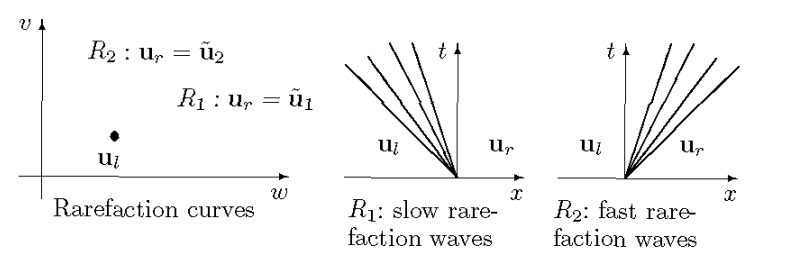
\includegraphics[width=.78\linewidth]{figures/p-system-rarefaction-curves-source.png}
\caption{}\label{fig:p-system-rarefaction-curves}
\end{figure}

对 $p$ 方程组, 不归一化特征向量更容易求解 \eqref{eq:rarefaction-curve-ode}. 得到曲线
\begin{equation}\label{eq:p-system-first-rarefaction-curve}
R_1:\quad\tilde{\bm{u}}_1(\gamma)=\begin{pmatrix}\tilde w_1(\gamma)\\\tilde v_1(\gamma)\end{pmatrix}:=\begin{pmatrix}w^l+\gamma\\v^l+\int_0^\gamma\sqrt{-p'(w^l+\xi)}\,\mathrm{d}\xi\end{pmatrix}
\end{equation}

\begin{equation}\label{eq:p-system-second-rarefaction-curve}
R_2:\quad\tilde{\bm{u}}_2(\gamma)=\begin{pmatrix}\tilde w_2(\gamma)\\\tilde v_2(\gamma)\end{pmatrix}:=\begin{pmatrix}w^l-\gamma\\v^l+\int_0^\gamma\sqrt{-p'(w^l-\xi)}\,\mathrm{d}\xi\end{pmatrix}.
\end{equation}


由于尚未归一化特征向量, 从稀疏曲线确定 $(w(x,t),v(x,t))$ 要略困难一些. 为计算 $\bm{u}^l$ 与 $\bm{u}^r$ 之间的 1-wave (其中 $\bm{u}^r$ 位于 $R_1$ 上), 取
\begin{equation}\label{eq:p-system-first-rarefaction-speed-range}
\lambda_1(\bm{u}^l)<\dfrac{x}{t}<\lambda_1(\bm{u}^r),
\end{equation}
并由方程
\begin{equation}\label{eq:p-system-first-rarefaction-volume}
\dfrac{x}{t}=\lambda_1=-\sqrt{-p'(w(x/t))}
\end{equation}
解出 $w(x/t)$. 然后令
\begin{equation}\label{eq:p-system-first-rarefaction-parameter}
\gamma=w(x/t)-w^l,
\end{equation}
并将其用于 \eqref{eq:p-system-first-rarefaction-curve}, 以确定 $v(x/t)$.

这里的图景与激波曲线的情形基本相同. 两条稀疏曲线都从左状态 $\bm{u}^l$ 出发; 它们与激波曲线具有相同的切向量 $\bm{r}_k$, 但沿相反方向传播. $R_1$ 曲线表示左状态与右状态的速度均为负的稀疏波 (有时称为慢波或后向波), 而 $R_2$ 曲线表示左状态与右状态的速度均为正的稀疏波 (快波或前向波).

\begin{figure}[H]
\centering
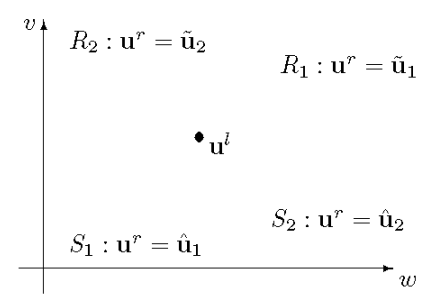
\includegraphics[width=.78\linewidth]{figures/slow-fast-state-curves-source.png}
\caption{慢曲线 $(S_1\cup R_1)$ 与快曲线 $(S_2\cup R_2)$.}\label{fig:slow-fast-state-curves}
\end{figure}

\paragraph*{一般解}

现在说明如何将激波与稀疏波组合起来, 得到 Riemann 问题的一般解. 基本定理如下.

\begin{Theorem}
\label{thm:local-riemann-solution}
假设守恒律方程组 \eqref{eq:conservation-law-system} 在状态空间的区域 $\Omega\subset\mathbb{R}^n$ 内严格双曲且真正非线性. 那么对任意 $\bm{u}^l\in\Omega$, 都存在 $\bm{u}^l$ 的邻域 $N\subset\Omega$, 使得只要 $\bm{u}^r\in N$, Riemann 问题 \eqref{eq:conservation-law-system}, \eqref{eq:riemann-piecewise-constant-data} 就存在弱解. 该解由至多 $n+1$ 个常数状态组成, 这些状态由稀疏波及满足 Lax 激波条件的激波分隔.
\end{Theorem}

不证明这一结果, 而是说明该过程如何在 $p$ 方程组的情形下实施. 从左状态 $\bm{u}^l$ 出发, 考虑由该点发出的两对激波曲线与稀疏曲线. 最好将它们看作两条 $C^1$ 曲线: 由 $S_1$ 和 $R_1$ 的并组成的"慢曲线" (慢激波与慢稀疏波), 以及由 $S_2$ 和 $R_2$ 的并组成的"快曲线". 当然, 若 Riemann 问题中的右状态 $\bm{u}^r$ 位于其中任一曲线上, 就可根据它位于原来四条曲线中的哪一条, 用单个波 (慢波或快波, 激波或稀疏波) 连接左状态与右状态. 剩下的问题是, 若右状态位于这些曲线划出的四个开区域之一, 会发生什么?

用一个快曲线族覆盖这四个区域, 即可得到解. 对通过 $\bm{u}^l$ 的慢曲线上的每个点 $\bar{\bm{u}}$, 都可构造曲线 $\bar S_2$ 和 $\bar R_2$. 这些新曲线分别表示激波与稀疏波, 都具有正速度, 并都以 $\bar{\bm{u}}$ 为左状态. 取 $\bar S_2$ 和 $\bar R_2$ 的并, 得到一个曲线族 (称为"快族"), 以原来慢曲线上的点 $\bar{\bm{u}}$ 为参数. 以下事实留作练习 (参见 Problem~\ref{ex:p-system-fast-family-covering}): 存在 $\bm{u}^l$ 的邻域 $\mathcal N$, 它被快族单值覆盖; 即对任意点 $\bm{u}^r\in\mathcal N$, 快族中恰有一个成员包含 $\bm{u}^r$.

\begin{figure}[H]
\centering
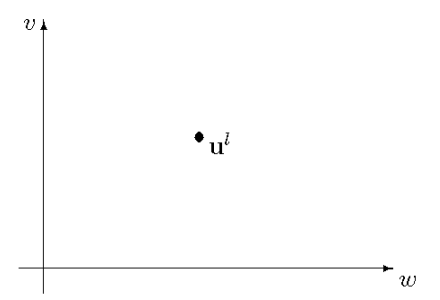
\includegraphics[width=.78\linewidth]{figures/slow-curve-fast-family-source.png}
\caption{慢曲线与快族.}\label{fig:slow-curve-fast-family}
\end{figure}

\begin{figure}[H]
\centering
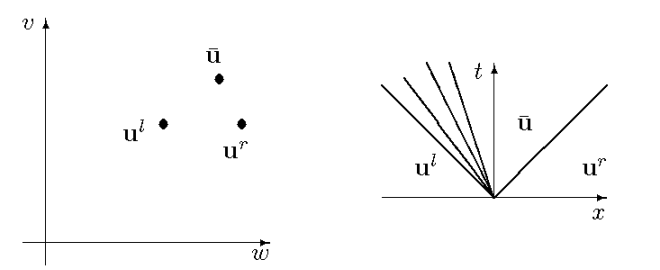
\includegraphics[width=.78\linewidth]{figures/slow-rarefaction-fast-shock-source.png}
\caption{慢稀疏波--快激波.}\label{fig:slow-rarefaction-fast-shock}
\end{figure}

\begin{figure}[H]
\centering
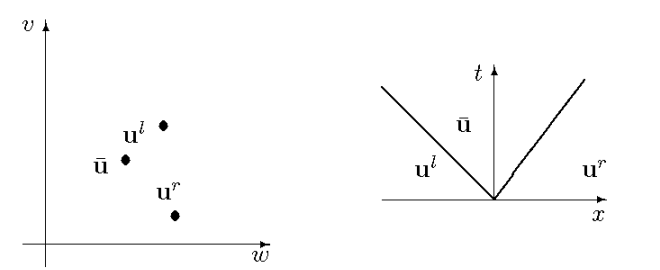
\includegraphics[width=.78\linewidth]{figures/slow-shock-fast-shock-source.png}
\caption{慢激波--快激波.}\label{fig:slow-shock-fast-shock}
\end{figure}

既然已利用左状态生成慢曲线与快族, Riemann 问题的求解就很简单了. 从任意右状态 $\bm{u}^r\in\mathcal N$ 出发, 只需沿快族中适当的成员返回慢曲线上的点 $\bar{\bm{u}}$. 现在将点 $\bar{\bm{u}}$ 作为两个波之间的中间状态: 一个慢波连接 $\bm{u}^l$ 与 $\bar{\bm{u}}$, 一个快波连接 $\bar{\bm{u}}$ 与 $\bm{u}^r$. 当然, 两个波中的每一个都可以是激波或稀疏波, 取决于右状态 $\bm{u}^r$ 位于原来的慢曲线与快曲线所界定的四个区域中的哪一个. 各种可能性见 Figures~\ref{fig:slow-rarefaction-fast-shock}--\ref{fig:slow-rarefaction-fast-rarefaction}.

\begin{figure}[H]
\centering
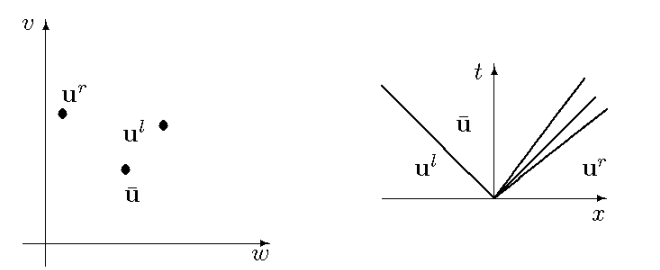
\includegraphics[width=.78\linewidth]{figures/slow-shock-fast-rarefaction-source.png}
\caption{慢激波--快稀疏波.}\label{fig:slow-shock-fast-rarefaction}
\end{figure}

\begin{figure}[H]
\centering
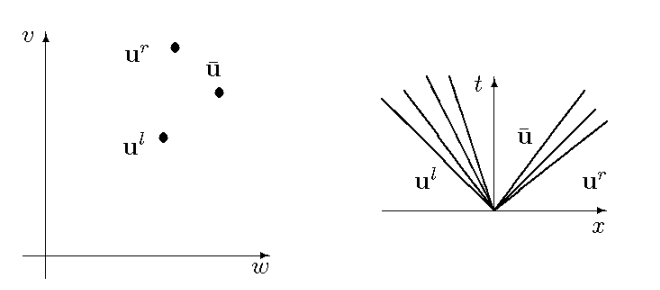
\includegraphics[width=.78\linewidth]{figures/slow-rarefaction-fast-rarefaction-source.png}
\caption{慢稀疏波--快稀疏波.}\label{fig:slow-rarefaction-fast-rarefaction}
\end{figure}
